\documentclass[tikz,border=4pt]{standalone}
\usepackage[T1]{fontenc}\usepackage[utf8]{inputenc}\usepackage{helvet}\renewcommand{\familydefault}{\sfdefault}
\usetikzlibrary{calc}
\begin{document}
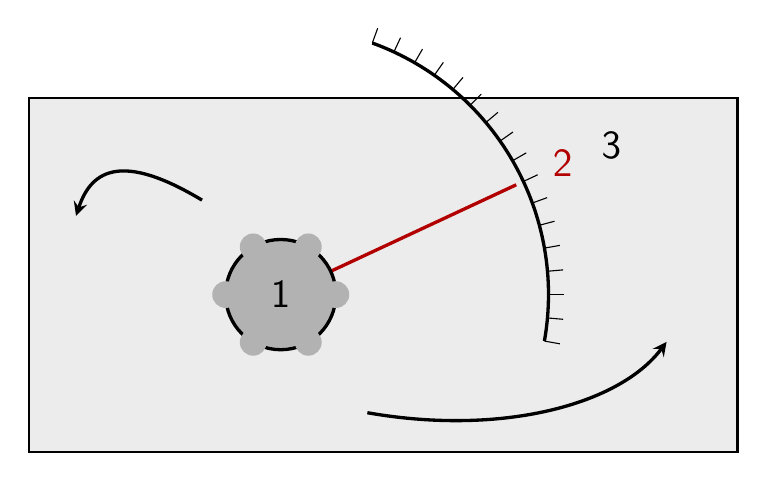
\begin{tikzpicture}[font=\Large,>=stealth]
\fill[gray!15] (0,0) rectangle (9,4.5); \draw[thick] (0,0) rectangle (9,4.5);
% Winkelskala 3
\draw[very thick] (3.2,2.0) ++(-10:3.4) arc (-10:70:3.4);
\foreach \a in {-10,-5,...,70}{\draw (3.2,2.0) ++(\a:3.4) -- ++(\a:0.2);}
\node at (7.4,3.9) {3};
% Zeiger 2
\draw[very thick,red!70!black] (3.2,2.0) -- ++(25:3.3); \node[red!70!black] at ($(3.2,2.0)+(25:3.95)$) {2};
% Verstellrad 1
\fill[gray!60] (3.2,2.0) circle (0.7); \draw[very thick] (3.2,2.0) circle (0.7);
\foreach \a in {0,60,...,300}{\fill[gray!60] (3.2,2.0) ++(\a:0.7) circle (0.17);}
\node at (3.2,2.0) {1};
\draw[->,very thick] (4.3,0.5) .. controls (6.0,0.2) and (7.5,0.6) .. (8.1,1.4);
\draw[->,very thick] (2.2,3.2) .. controls (1.2,3.8) and (0.8,3.6) .. (0.6,3.0);
\end{tikzpicture}
\end{document}
